% =====================================================================
%  Sexism Identification in Memes  --  EXIST 2026 Lab Project
%  Author: Klaudia Banasiewicz
%
%  Compile with pdflatex (run twice for references). Standard packages only.
% =====================================================================
\documentclass[11pt,a4paper]{article}

\usepackage[utf8]{inputenc}
\usepackage[T1]{fontenc}
\usepackage[margin=2.4cm]{geometry}
\usepackage{graphicx}
\usepackage{booktabs}
\usepackage{amsmath}
\usepackage{array}
\usepackage{multirow}
\usepackage{float}      % provides the [H] specifier to lock floats in place
\usepackage{xcolor}
\usepackage{caption}
\usepackage[hidelinks]{hyperref}

\graphicspath{{../project/figures/}}

\captionsetup{font=small,labelfont=bf}
\setlength{\parskip}{2pt}

\title{\textbf{Sexism Identification in Memes}\\[2pt]
\large A multimodal study with text, image and physiological signals (EXIST 2026)}
\author{Klaudia Banasiewicz}
\date{}

\begin{document}
\maketitle
\vspace{-1.2em}

% =====================================================================
\section{Introduction}
% =====================================================================
Memes are hard to moderate automatically: the offensive part is often split between a short
caption and an image that looks harmless on its own. The EXIST 2026 ``Sexism in Memes'' lab~\cite{exist}
splits this into three related tasks. Task~2.1 asks whether a meme is sexist at all
(\textsc{yes}/\textsc{no}); Task~2.2 asks, if it is, what \emph{kind} of sexism it shows
(\textsc{direct} vs.\ \textsc{judgemental}); and Task~2.3 asks which of five detailed
\emph{categories} apply, which is a multi-label problem.

What makes this dataset unusual is that the organisers released more than just the memes and
their labels. While volunteers annotated the memes, their physical reactions were recorded with
three sensors: eye-tracking, heart rate, and EEG. So for each meme the dataset also gives a
summary of how real people reacted to the image. This leads to the main question of the project:
\emph{does that physical signal tell us anything about sexism that the text and image do not
already tell us?} The report describes the models I tried, the systems I finally submitted, the
cross-validation results, and most importantly the comparison of performance with and without
physiological data.

% =====================================================================
\section{Dataset and preprocessing}
% =====================================================================
The training set contains 3{,}984 memes and the test set 1{,}053, split almost evenly between
English (2{,}005) and Spanish (1{,}979). Every meme is annotated by six people. Hard labels are
taken as the majority vote over the six annotators and soft labels as the vote fractions. For
Task~2.2 the raw ``\,-\,'' annotation is mapped to
\textsc{no}, and for Task~2.3 the per-annotator category lists are turned into a multi-label
vector (a category is kept if more than half of the annotators chose it, with a top-1 fallback).
Table~\ref{tab:dist} shows the resulting class distributions, which are very imbalanced. This
imbalance drives most of my modelling choices later.

\begin{table}[H]
\centering
\small
\caption{Hard-label class distribution in the training set (3{,}984 memes).
Task~2.3 counts are multi-label, so they sum to more than 3{,}984.}
\label{tab:dist}
\begin{tabular}{llr}
\toprule
Task & Class & Count \\
\midrule
2.1 (binary) & \textsc{yes} / \textsc{no} & 2{,}286 / 1{,}698 \\
\midrule
2.2 (type)   & \textsc{no}          & 1{,}968 \\
             & \textsc{direct}      & 1{,}474 \\
             & \textsc{judgemental} & \phantom{0}542 ($\approx$14\%) \\
\midrule
2.3 (category) & objectification              & 597 \\
               & stereotyping-dominance       & 591 \\
               & ideological-inequality       & 544 \\
               & sexual-violence              & 232 \\
               & misogyny-non-sexual-violence & 118 \\
\bottomrule
\end{tabular}
\end{table}

\paragraph{Text.} The caption is used as raw text and tokenised on the fly with the XLM-RoBERTa~\cite{xlmr}
tokeniser, truncated to 128 tokens. XLM-R is multilingual, so the same model handles both English
and Spanish without a separate per-language pipeline.

\paragraph{Image.} Each meme image is encoded once with a frozen CLIP~\cite{clip} image encoder into a
512-dimensional vector. CLIP is not fine-tuned; its embedding is treated as a fixed feature.

\paragraph{Physiological.} For each meme the dataset provides three modalities recorded from the
viewers: eye-tracking (pupil-diameter and reaction-time statistics, 24 features per viewer),
heart rate (4 features), and EEG (band-power per channel, 80 features). These are
aggregated across the viewers of a meme into a single 104-dimensional vector. The model never sees
raw EEG traces --- only this compact summary. The image, sensorial and text features are precomputed
once and re-aligned to each record by meme ID before use.

% =====================================================================
\section{Models and experiments}
% =====================================================================
I started from simple baselines and built up to a multimodal late-fusion system. The three tasks
share the same overall setup, but I adapt it to each task's difficulty and imbalance.

\subsection{Baselines}
I use two kinds of baseline for comparison. The first are the competition's \emph{majority} and
\emph{minority} class predictors (always output the most/least frequent label). The second is a
plain XLM-RoBERTa-base trained in the most basic way, one per task, with no oversampling,
no fusion and none of the extra techniques I add later. These plain models are my reference point:
they show how much each later change actually improves the results.

\subsection{Text backbones: XLM-RoBERTa}
The text model in every final system is XLM-RoBERTa. For Task~2.1 I do a full fine-tune of the
\emph{large} variant (all weights updated, 3 epochs, learning rate $1\!\times\!10^{-5}$,
class-weighted cross-entropy, bf16 + gradient checkpointing to fit on one GPU). The large model
plus class weighting does most of the work here; fusion only adds a small improvement.

Task~2.2 is harder because \textsc{judgemental} is only $\approx$14\% of the data. A full
fine-tune on the rebalanced data was unstable, so I switched to \textbf{LoRA}~\cite{lora} (low-rank adapters,
$r{=}16$, $\alpha{=}32$ on the query/value projections) with the backbone frozen, which trains far
more stably. On top of that I use two ways to handle the imbalance: \textbf{oversampling} the minority
classes up to the majority count (training split only), and \textbf{focal loss}~\cite{focal} ($\gamma{=}2$),
which makes training focus on the hard, rare examples instead of the easy ones.

Task~2.3 is multi-label, so a single softmax head is the wrong tool: a single-label XLM-R-base
simply learns to always predict \textsc{no} and never fires any category head. Instead I use
\textbf{five independent sigmoid heads} trained with binary cross-entropy and a per-category
positive-class weight (the negative/positive ratio), so rare categories get a stronger gradient.
A category fires above $0.5$; if none fires, the top-scoring one is kept so the model never
predicts ``nothing.''

\subsection{Multimodal late fusion}
Image and physiological information enter through a separate and very simple branch: a
logistic regression (standardised features, regularisation $C=1.0$) trained on the concatenated
image\,$\oplus$\,sensorial vector (512 + 104 = 616 dimensions). At inference the two branches vote
at the probability level (late fusion~\cite{latefusion}),
\[
p \;=\; \alpha\, p_{\text{text}} \;+\; (1-\alpha)\, p_{\text{img+sens}},
\]
with $\alpha$ swept on a held-out validation split. Task~2.1 selected $\alpha=0.95$ (text
dominates) and Task~2.2 $\alpha=0.75$. Task~2.3 is not $\alpha$-fused but \emph{gated}: if the
Task~2.1 head says \textsc{no}, the output is simply \textsc{no}; otherwise the five category
heads decide, and the soft scores are multiplied by $p(\textsc{yes})$ so the probabilities stay
consistent. Figure~\ref{fig:arch} shows this pipeline.

\begin{figure}[H]
\centering
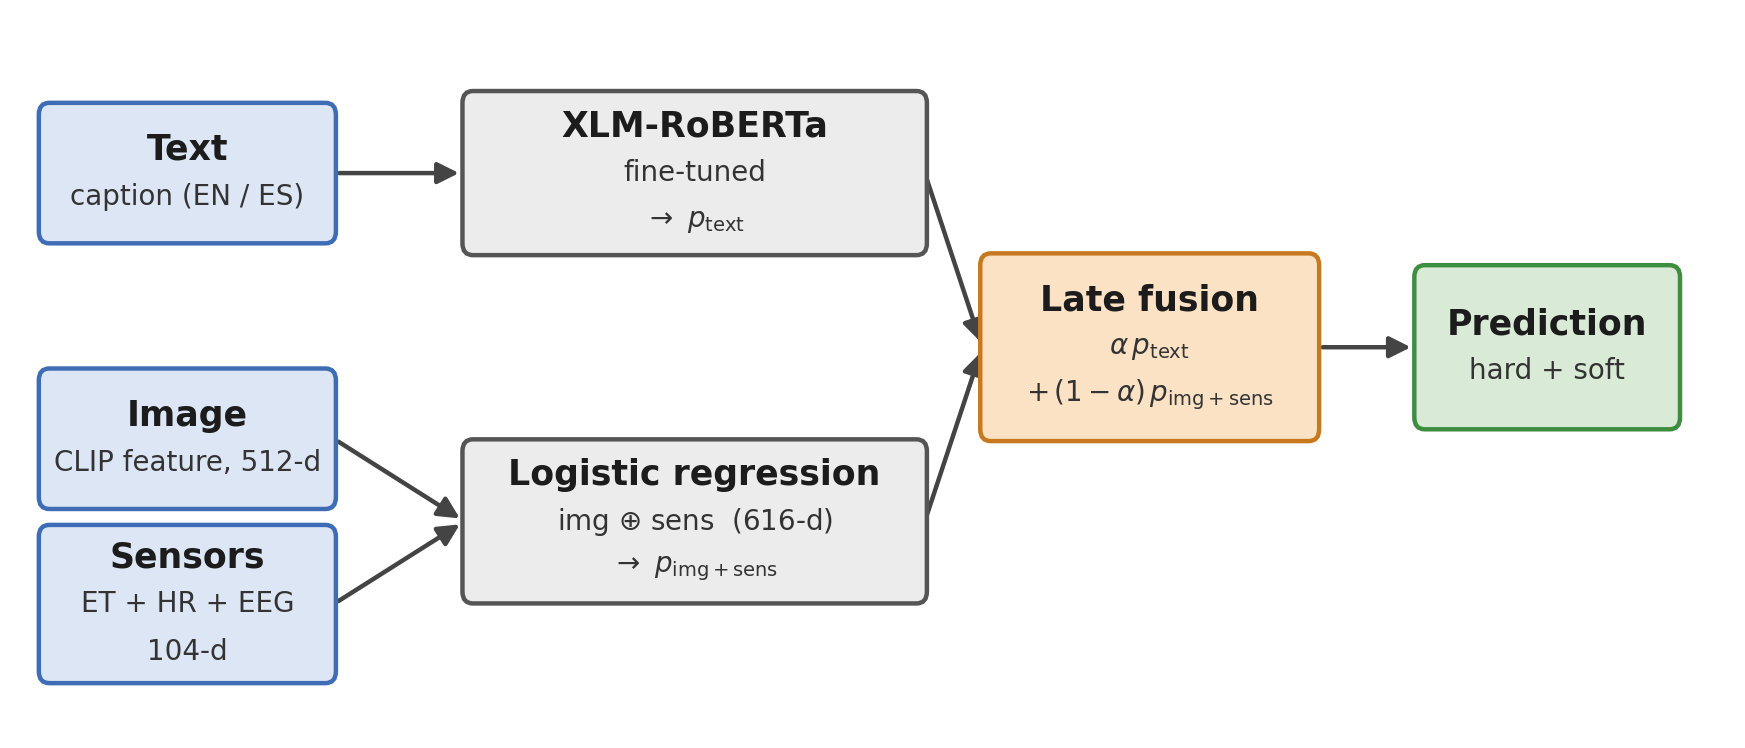
\includegraphics[width=\linewidth]{fusion_architecture.png}
\caption{Late-fusion architecture shared by the three tasks. The text model and a linear
image+sensor model each produce a probability; these are combined with a tuned weight $\alpha$
(Task~2.3 instead gates the category heads on the Task~2.1 decision).}
\label{fig:arch}
\end{figure}

\subsection{The controlled modality experiment}
The late-fusion system above is good for submission but bad for answering ``do sensors help'',
because too many things differ between configurations. For a fair comparison I used one fixed
small fusion MLP and 5-fold cross-validation,
changing \emph{only} the input features: text embeddings alone, text + image, and
text + image + physiological. Same model, same folds, only the inputs change. This is the
experiment that Section~\ref{sec:results} is based on.

% =====================================================================
\section{Experimental results}
\label{sec:results}
% =====================================================================
Two evaluations are reported. The 5-fold cross-validation (Table~\ref{tab:cv}) is the
\emph{generalisation} estimate and the basis for the physiological-data comparison. The
training-set evaluation (Table~\ref{tab:bvf}) is in-sample and therefore optimistic; it is useful
for showing the relative effect of each modelling change, but its absolute numbers should not be
read as test performance. The official lab metric is ICM / ICM-Soft via PyEvALL; during development
I used macro-F1 to compare and choose between models.

\subsection{With vs.\ without physiological data}
Table~\ref{tab:cv} reports 5-fold macro-F1 (mean $\pm$ std) for the three feature configurations,
from the controlled modality experiment; Figure~\ref{fig:cv} shows the same data per fold.

\begin{table}[H]
\centering
\small
\caption{5-fold cross-validation macro-F1 (mean\,$\pm$\,std). Same fusion MLP and folds for every
row --- only the input features change. \textbf{Bold} = best configuration per task.}
\label{tab:cv}
\begin{tabular}{lccc}
\toprule
Features & Task~2.1 & Task~2.2 & Task~2.3 \\
\midrule
Text only            & \textbf{0.590\,$\pm$\,0.009} & 0.385\,$\pm$\,0.019 & 0.237\,$\pm$\,0.017 \\
Text + Image         & 0.581\,$\pm$\,0.010 & \textbf{0.398\,$\pm$\,0.006} & 0.246\,$\pm$\,0.015 \\
Text + Image + Phys  & 0.578\,$\pm$\,0.011 & 0.394\,$\pm$\,0.008 & \textbf{0.253\,$\pm$\,0.013} \\
\bottomrule
\end{tabular}
\end{table}

\begin{figure}[H]
\centering
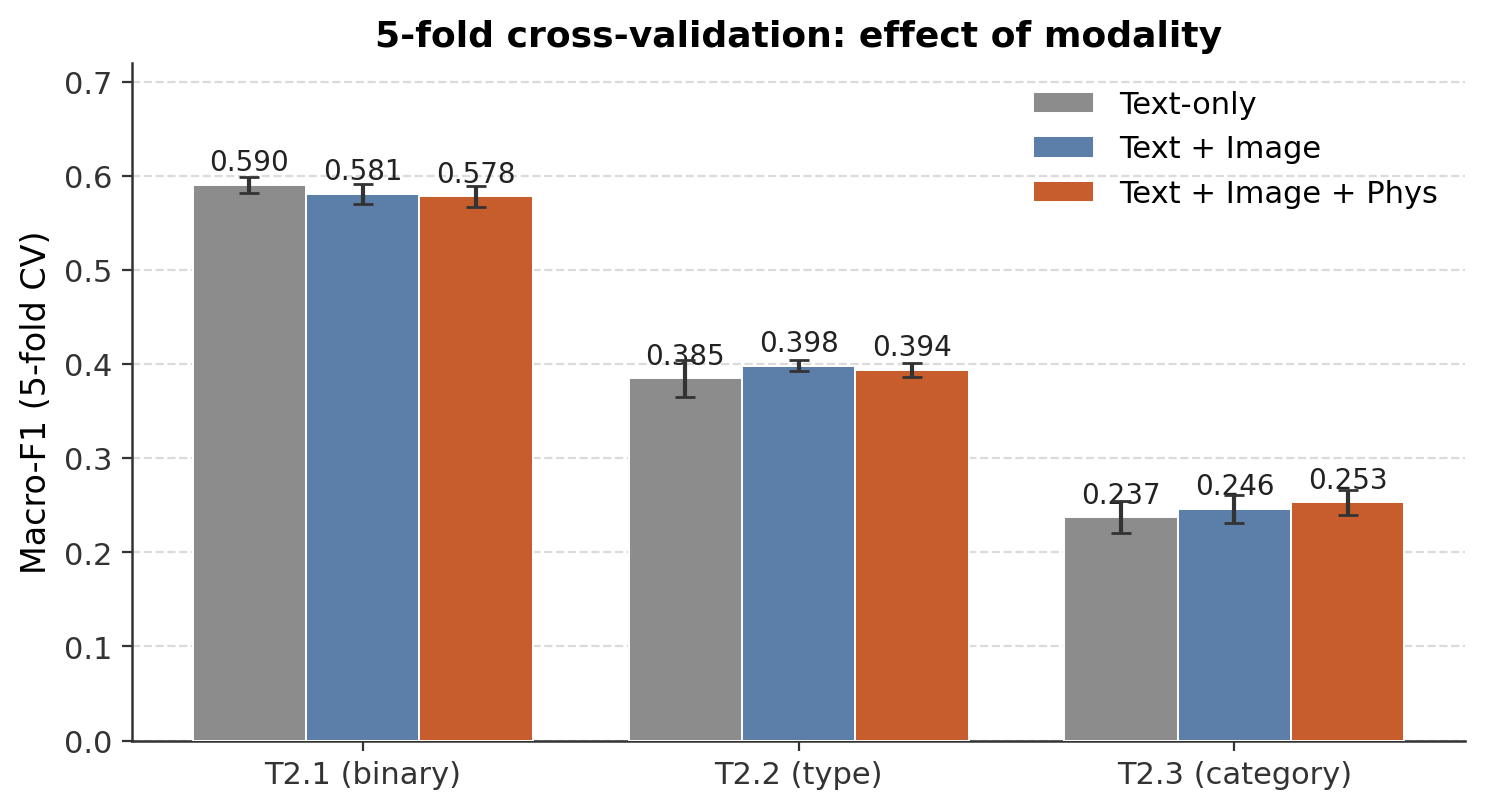
\includegraphics[width=0.82\linewidth]{cv_phys_comparison.png}
\caption{5-fold cross-validation by modality. Error bars are the across-fold standard deviation.
Physiological data only helps Task~2.3.}
\label{fig:cv}
\end{figure}

The pattern is clear and, to me, the most interesting result of the project:
\begin{itemize}\setlength{\itemsep}{1pt}
\item \textbf{Task~2.1 (binary):} physiological data does \emph{not} help. Text alone is best
(0.590); adding image and then sensors slightly \emph{lowers} macro-F1 (to 0.578). Deciding
\emph{whether} a meme is sexist is mostly a text decision, and the extra inputs mostly add noise.
\item \textbf{Task~2.2 (type):} essentially flat. The CLIP image features give a small lift over
text (0.385\,$\rightarrow$\,0.398), but adding physiological data on top changes nothing within
the noise (0.394). Whatever the sensors carry here is already captured by the image.
\item \textbf{Task~2.3 (category):} the one positive case. Physiological data raises macro-F1 from
0.246 (text+image) to 0.253, about $+0.016$ over text-only --- small in absolute terms but
consistent across all five folds. This is the hardest, most imbalanced task, and it is exactly
where the rarest categories have the least text to learn from.
\end{itemize}
The take-away is that physiological signals only help where text alone is already near its limit
and the classes are very imbalanced (the detailed categories), and even there the gain is small.

\subsection{Final systems vs.\ baselines}
Table~\ref{tab:bvf} compares the plain XLM-R-base text baseline with the final per-task system on
the full training set (macro-F1 / accuracy / AUC), reproducing the numbers behind the project's
comparison figures.

\begin{table}[H]
\centering
\small
\caption{Text-only baseline vs.\ final system, measured on the full training set (3{,}984 memes).}
\label{tab:bvf}
\begin{tabular}{llccc}
\toprule
Task & System & Macro-F1 & Acc. & AUC \\
\midrule
\multirow{2}{*}{2.1} & XLM-R-base (text)        & 0.422 & 0.591 & 0.386 \\
                     & XLM-R-large + fusion     & \textbf{0.794} & \textbf{0.797} & \textbf{0.867} \\
\midrule
\multirow{2}{*}{2.2} & XLM-R-base (text)        & 0.435 & 0.608 & 0.741 \\
                     & XLM-R-large + LoRA + fusion & \textbf{0.635} & \textbf{0.674} & \textbf{0.827} \\
\midrule
\multirow{2}{*}{2.3} & XLM-R-base single-label  & 0.000 & 0.895 & 0.614 \\
                     & XLM-R-base multi-label   & \textbf{0.357} & 0.724 & \textbf{0.821} \\
\bottomrule
\end{tabular}
\end{table}

The single-label Task~2.3 baseline scores 0.895 accuracy yet \textbf{0.000} macro-F1: it predicts
\textsc{no} for everything and is ``right'' most of the time precisely because most memes carry no
category --- a clear reason to trust macro-F1 instead of accuracy on imbalanced data. The multi-label
head recovers every category (Table~\ref{tab:cat}); the scores are highest on the common categories
and lowest on the rarest (\emph{sexual-violence}, \emph{misogyny-NSV}), which simply have very few
training examples.

\begin{table}[H]
\centering
\small
\caption{Per-category F1 of the multi-label model on Task~2.3 (training set).}
\label{tab:cat}
\begin{tabular}{lc}
\toprule
Category & F1 \\
\midrule
Ideological inequality        & 0.546 \\
Stereotyping dominance        & 0.392 \\
Objectification               & 0.341 \\
Sexual violence               & 0.285 \\
Misogyny (non-sexual violence)& 0.223 \\
\midrule
\textbf{Macro average}        & \textbf{0.357} \\
\bottomrule
\end{tabular}
\end{table}

\subsection{Test-set behaviour}
On the 1{,}053 test memes the final systems produce label distributions close to the training
frequencies, which is a basic sanity check that nothing collapsed: Task~2.1 predicts 580 \textsc{yes}
/ 473 \textsc{no}; Task~2.2 predicts 458 \textsc{no} / 346 \textsc{direct} / 249 \textsc{judgemental};
and all five Task~2.3 categories appear (objectification 293, stereotyping 274, ideological 265,
misogyny-NSV 152, sexual-violence 132). No category degenerates to zero at test time.

% =====================================================================
\section{Final model selection}
\label{sec:final}
% =====================================================================
The submitted systems are the three in the lower rows of Table~\ref{tab:bvf}: XLM-R-large full
fine-tune + fusion for Task~2.1, XLM-R-large + LoRA + oversampling + focal loss + fusion for
Task~2.2, and XLM-R-base multi-label (gated by Task~2.1) for Task~2.3. They were chosen on
held-out validation macro-F1, and they all fit on a single GPU and share one ``two models that
vote'' structure, which kept the implementation and the test-time pipeline simple. Physiological
data was kept only for Task~2.3, where the cross-validation supported it; for the other two tasks
the fusion branch mainly contributes the image features.

% =====================================================================
\section{Conclusion}
% =====================================================================
The clearest lesson is about \emph{where} multimodality helps. For sexism in memes, text is by far
the strongest signal; scaling XLM-R-base to large and handling class imbalance (class weights, LoRA,
focal loss, oversampling, multi-label sigmoid heads) accounts for almost all of the improvement.
Image features add a little, and physiological signals --- the most unusual part of this dataset ---
helped only on the hardest, most imbalanced task (the detailed categories), and only by a small but
steady amount. This is a useful, if a bit disappointing, result: collecting EEG, eye-tracking and
heart-rate data did not help with simple yes/no sexism detection.

If I had more time, the next steps would be the ones the cross-validation points to: replace the
frozen CLIP + logistic-regression branch with a proper vision--language model (for example
Qwen2.5-VL), add a small attention layer over the 104 physiological features
instead of feeding them in as a flat list, and try stronger regularisation and per-language
(EN / ES) fine-tuning. The current systems are a solid baseline for all three tasks, and the
modality study is the part I would most like to build on.

% =====================================================================
% References. These are the actual methods used in the project --- not
% hallucinated. Bibliographic details kept standard/minimal.
% =====================================================================
\begin{thebibliography}{9}\small
\bibitem{xlmr} A.\ Conneau et al., ``Unsupervised Cross-lingual Representation Learning at Scale
(XLM-R),'' \emph{ACL}, 2020.
\bibitem{clip} A.\ Radford et al., ``Learning Transferable Visual Models from Natural Language
Supervision (CLIP),'' \emph{ICML}, 2021.
\bibitem{lora} E.\ Hu et al., ``LoRA: Low-Rank Adaptation of Large Language Models,''
\emph{ICLR}, 2022.
\bibitem{focal} T.-Y.\ Lin et al., ``Focal Loss for Dense Object Detection,''
\emph{ICCV}, 2017.
\bibitem{latefusion} C.~G.~M.\ Snoek, M.\ Worring, and A.~W.~M.\ Smeulders, ``Early versus Late
Fusion in Semantic Video Analysis,'' \emph{ACM Multimedia}, 2005.
\bibitem{exist} EXIST 2026 Lab, ``Sexism Identification in Memes --- Lab Guidelines and PyEvALL
evaluation framework.''
\end{thebibliography}

\end{document}
